\documentclass[a4paper, 12pt]{article}
\usepackage[english]{babel}
\usepackage{fullpage}
\usepackage{pgf}
\usepackage{tikz}
\usepackage{hyperref}  % makes cross references and URLs clickable
\newcommand{\code}[1]{\texttt{#1}}
\newcommand{\link}[1]{\hyperref[#1]{#1}} % links to sections
\usepackage[overload]{textcase}
\newcommand{\codeHook}[1]{\mbox{\ttfamily\MakeTextUppercase{#1}}}
\usepackage{listings}
\usepackage{color}
\definecolor{light-gray}{gray}{0.95}
\usepackage{textcomp}
% set listings as in other WR-doc(s)
\lstset{columns=flexible, upquote=true,  frame=single, captionpos=b, caption=, basicstyle=\scriptsize, backgroundcolor=\color{light-gray}, label=lst:init_src}
\usepackage{longtable} % table over many pages
\usepackage[document]{ragged2e} %texta djustment
\usepackage{mdwlist} % to have tight itemization
\usepackage[T1]{fontenc}
\usepackage{lmodern}
%%%%%%%%%%%%%%%%%%%%%%%%%%%%%%%%%%%%

\begin{document}

\title{White Rabbit PTP Core User's Manual}
\author{Grzegorz Daniluk\\ CERN BE-CO-HT}

\raggedright
{\LARGE {\bf White Rabbit PTP Core User's Manual}}\\[0.2 cm]
\hrule height 4pt \vspace{0.1cm}
\raggedleft
{\large \today ~ ( \input{version})}\\
{\large Building and Running}\\
\vspace*{\fill}
\raggedright
{\large Grzegorz Daniluk (CERN BE-CO-HT)}\\
\hrule height 2pt
\justify

\newpage

\tableofcontents

\newpage

{\noindent \LARGE {\bf Introduction}}\\


This is the user manual for the White Rabbit PTP Core, part of the White
Rabbit project. It describes the building and running process. If you don't
want to get your hands dirty and prefer to start with the demo binaries
available at \url{http://www.ohwr.org/projects/wr-cores/files} please skip
section \ref{Building the Core} and move forward directly to section
\ref{Running and Configuring}.


% ##########################################################################
\section{Software and hardware requirements}
\label{Software and hardware requirements}

% ==========================================================================
\subsection{Repositories and Releases}
\label{Repositories and Releases}

This manual is about the official \input{version} stable release of the White
Rabbit PTP Core (\codeHook{WRPC}).
The code and documentation for the project is distributed in the
following places:

\begin{itemize*}

\item \url{http://www.ohwr.org/projects/wr-cores/documents}

	hosts the pdf documentation for every official release.

\item \url{http://www.ohwr.org/projects/wr-cores/files}

	place where you can find a synthesized bitstream, ready to be downloaded to
  SPEC, for every stable release

\item \url{git://ohwr.org/hdl-core-lib/wr-cores.git}

	read-only repository with complete HDL sources of the \codeHook{WRPC}

\item \url{git://ohwr.org/hdl-core-lib/wr-cores/wrpc-sw.git}

  read-only repository with the \codeHook{WRPC} \codeHook{LM32} software

\end{itemize*}
Other tools useful for building and running the \codeHook{WRPC} can be downloaded from
the following locations:

\begin{itemize*}

\item \url{git://ohwr.org/misc/hdl-make.git}

  \textit{hdlmake} is used in the HDL synthesis process to create a Makefile based
on the set of Manifest files.

\item \url{http://www.ohwr.org/attachments/download/1133/lm32.tar.xz}

  \codeHook{LM32} toolchain used to compile the \codeHook{WRPC} software

\end{itemize*}
Repositories containing the \codeHook{WRPC} gateware and software (\textit{wr-cores},
\textit{wrpc-sw}) are tagged with \codeHook{wrpc-v3.0} tag. Other tools
used to build the core and load it into \codeHook{SPEC} board should be used in their
newest stable releases.


% ==========================================================================
\subsection{Required hardware}
\label{Required hardware}

The absolute minimum to run the \codeHook{wr ptp core} is a PC computer with
Linux and a Simple PCIe \codeHook{fmc} Carrier
(\codeHook{spec}) - \url{http://www.ohwr.org/projects/spec}. However, it is highly
recommended to use also the \codeHook{dio} \codeHook{fmc} card (\url{http://www.ohwr.org/projects/fmc-dio-5chttla})
to be able to feed 1-PPS and 10MHz from external clock and output 1-PPS aligned
to the WR time. To test the White Rabbit synchronization, you will also need:
\begin{itemize*}
\item another \codeHook{spec} board with a \codeHook{dio} \codeHook{fmc} or a White Rabbit Switch;
\item pair of \codeHook{wr}-supported \codeHook{sfp} transceivers (the list of supported
\codeHook{sfp}s can be found on our wiki page \url{http://www.ohwr.org/projects/white-rabbit/wiki/SFP})
\item a roll of G652, single mode fiber to connect your \codeHook{spec}s or \codeHook{spec}
with a \codeHook{wr} Switch.
\end{itemize*}

% ##########################################################################
\section{Building the Core}
\label{Building the Core}

\textbf{Note:} you can skip this chapter if you want to use the release binaries
available from \textit{ohwr.org}.

\vspace{1em}
Building the core is a two step process. First you have to
synthesize the FPGA firmware (gateware) and then compile the software which
will be executed by the \codeHook{lm32} soft-core processor. If you don't need to
modify the \codeHook{lm32} software, you can skip the compilation stage since
synthesized gateware already embeds the default software for the release.

% ==========================================================================
\subsection{HDL synthesis}
\label{HDL synthesis}

Before running the synthesis process you have to make sure your environment is
set up correctly. You need a Xilinx ISE software with at least a WebPack
license. \textit{ISE} provides a set of scripts: \textit{settings32.sh},
\textit{settings32.csh}, \textit{settings64.sh} and \textit{settings64.csh} that configure all
the system variables required by the Xilinx software. Depending on a shell you
use and whether your Linux is 32 or 64-bits you should execute one of them
before the other tools are used. For 64-bit system and BASH shell you should
call:
\begin{lstlisting}
/opt/Xilinx/<version>/ISE_DS/settings64.sh
\end{lstlisting}

The easiest way to ensure that \textit{ISE}-related variables are always set in your
shell is adding the execution of the script to your \textit{bash.rc} file. You can
check if the shell is configured correctly by verifying if the \textit{\$XILINX}
variable contains path to your \textit{ISE} installation directory.

\textbf{Note:} current version of \textit{hdlmake} tool developed at CERN requires
modification of \textit{\$XILINX} variable after \textit{settings} script execution.
This (provided that the installation path for \textit{ISE} is /opt/Xilinx/<version>)
should be the following:

\begin{lstlisting}
$ export XILINX=/opt/Xilinx/<version>/ISE_DS
\end{lstlisting}

\textbf{Note:} the Xilinx project file included in the \codeHook{wrpc} sources was created
with Xilinx ISE 14.5. It is however recommended to use the newest available
version of the ISE software.

\vspace{1em}
HDL sources for the \codeHook{wr ptp core} could be synthesized using Xilinx ISE without
any additional tools, but using \textit{hdlmake} is more convenient. It creates a
synthesis Makefile and ISE project file based on a set of Manifest.py files
deployed among the directories inside the \textit{wr-cores} repository.

First, please clone the \textit{hdlmake} repository from its location given in
section \ref{Repositories and Releases}:\newpage
\begin{lstlisting}
$ wget http://www.ohwr.org/attachments/download/2070/hdlmake-v1.0
$ git clone git://ohwr.org/misc/hdl-make.git <your_location>/hdl-make
$ cd <your_location>/hdl-make
$ git checkout 9d303ee
\end{lstlisting}

Then, using your favorite editor, you should create an \textit{hdlmake} script in
/usr/bin to be able to call it from any directory. The script should have the
following content:
\begin{lstlisting}
#!/usr/bin/env bash
python2.7 /path_to_hdlmake_sources/hdl-make/hdlmake/__main__.py #@
\end{lstlisting}

After that, you should make your script executable:
\begin{lstlisting}
chmod a+x /usr/bin/hdlmake
\end{lstlisting}

\vspace{1em}
Having Xilinx ISE software and \textit{hdlmake} in place, you can clone the main
\codeHook{wr ptp core} git repository and start building the FPGA bitstream.
First, please create a local copy of the \textit{wr-cores}:
\begin{lstlisting}
$ git clone git://ohwr.org/hdl-core-lib/wr-cores.git <your_location>/wr-cores
$ cd <your_location>/wr-cores
\end{lstlisting}

To build the gateware using sources of a stable release wrpc-v3.0, you
have to checkout the proper git tag:

\begin{lstlisting}
$ git checkout wrpc-v3.0
\end{lstlisting}

If you use \textit{wr-cores} within another project (like \textit{wr-nic}), you may need
to check out another release tag for this repository. Please refer to the
project's documentation to find out which version of this package you need to
build.

You also need to fetch other git repositories containing modules instantiated
inside the \codeHook{wr ptp core} HDL. They are configured as git submodules:
\begin{lstlisting}
$ git submodule init
$ git submodule update
\end{lstlisting}

The local copies of the submodules are stored to:

\begin{lstlisting}
<your_location>/wr-cores/ip_cores
\end{lstlisting}

\vspace{1em}
The subdirectory which contains the main synthesis Manifest.py for \codeHook{spec} board
and in which you should perform the whole process is:

\begin{lstlisting}
$ cd <your_location>/wr-cores/syn/spec_1_1/wr_core_demo/
\end{lstlisting}

First, please call \textit{hdlmake} to create synthesis Makefile for Xilinx
ISE:

\begin{lstlisting}
$ hdlmake
\end{lstlisting}

After that, the actual synthesis is just the matter of executing:

\begin{lstlisting}
$ make
\end{lstlisting}

This takes (depending on your computer speed) about 15 minutes and should create
two files with FPGA firmware: \textit{spec\_top.bit} and \textit{spec\_top.bin}. The
former can be downloaded to FPGA with Xilinx Platform Cable using e.g.
\textit{Xilinx Impact}. The latter can be used with kernel drivers from the
\textit{spec-sw} repository (check example in section \ref{Running and
Configuring}).

\vspace{1em}
If, on the other hand, you would like to clean-up the repository and rebuild
everything from scratch you can use the following commands:
\begin{itemize*}
\item \textit{\$ make clean} - removes all synthesis reports and log files;
\item \textit{\$ make mrproper} - removes spec\_top.bin and spec\_top.bit files;
\end{itemize*}

% ==========================================================================
\subsection{LM32 software compilation}
\label{LM32 software compilation}

\textbf{Note:} By default, the \codeHook{lm32} software for a stable release is embedded
inside the FPGA bitstream you've downloaded from \textit{ohwr.org} or synthesized in
the previous step. This means you don't have to do a manual compilation of the
\codeHook{lm32} software unless you want to use a development version or you've made
some changes required by your application.

\vspace{1em}
To compile the \codeHook{lm32} software for the White Rabbit \codeHook{ptp} Core you will
need to download and unpack the \codeHook{lm32} toolchain from the location mentioned
in section \ref{Repositories and Releases}:

\begin{lstlisting}
$ wget http://www.ohwr.org/attachments/download/1133/lm32.tar.xz
$ tar xJf lm32.tar.xz -C <your_lm32_location>
\end{lstlisting}

Then you need to set a \texttt{CROSS\_COMPILE} variable in order
to compile the software for the \codeHook{lm32} processor:

\begin{lstlisting}
$ export CROSS_COMPILE="<your_lm32_location>/lm32/bin/lm32-elf-"
\end{lstlisting}

To get the sources of the \codeHook{wrpc} software please clone the \textit{wrpc-sw} git
repository tagged with wrpc-v3.0 tag. If you use \codeHook{wrpc} within another
project, you may need to checkout a different tag or a specific commit. If this
applies, please refer to a documentation for this project.

\begin{lstlisting}
$ git clone git://ohwr.org/hdl-core-lib/wr-cores/wrpc-sw.git <your_location>/wrpc-sw
$ cd <your_location>/wrpc-sw
$ git checkout wrpc-v3.0   # or "git checkout master"
\end{lstlisting}

Before you can compile \textit{wrpc-sw} you need to make a few configuration choices.
The package uses \textit{Kconfig} as a configuration engine, so you may run one of the
following commnads (the first is text-mode, the second uses a KDE GUI
and the third uses a Gnome GUI):

\begin{lstlisting}
$ make menuconfig
$ make xconfig
$ make gconfig
\end{lstlisting}

Other \textit{Kconfig} target applies, like \code{config}, \code{oldconfig}
and so on.  A few default known-good configurations are found in
\texttt{./configs} and you choose one by \textit{make}ing it by name:

\begin{lstlisting}
$ make spec_defconfig
\end{lstlisting}

The most important configuration choice at this point in time is
whether to enable Etherbone or not. It is disabled by default in
\code{spec\_defconfig} and enabled by default in
\code{etherbone\_defconfig}.

After the package is configured, just run \code{make} without
parameters to build your binary file:

\begin{lstlisting}
$ make
\end{lstlisting}

The first time you build, the \textit{Makefile} automatically downloads
the \textit{git submodules} of this package, unless you already did that
by hand. The second and later build won't download anything
from the network.

The resulting binary \textit{wrc.bin} can be then used with the loader from
\textit{spec-sw} software package to program the \codeHook{lm32} inside the White Rabbit \codeHook{ptp}
Core (section \ref{Running and Configuring}).

% ##########################################################################
\section{Running and Configuring}
\label{Running and Configuring}

% ==========================================================================
\subsection{Downloading firmware to SPEC}
\label{Downloading firmware to SPEC}

For this step you will need a \codeHook{spec} board software support package
(\codeHook{spec-sw}) from \textit{ohwr.org}. It is a set of Linux kernel drivers and
userspace tools, that interact with a \codeHook{spec} board plugged into PCI-Express
slot.

Instructions in this section are based on a development version of \codeHook{spec-sw}
so if a stable release more recent than \textit{2014-02} is available, you should
use it instead. 

If there is a more recent version of the \codeHook{spec} software support, the
up-to-date documentation can always be found in \textit{doc/} subdirectory of
\codeHook{spec-sw} git repository.

\vspace{1em}
First, please clone the git repository of \codeHook{spec-sw} package and build it:

\begin{lstlisting}
$ git clone git://ohwr.org/fmc-projects/spec/spec-sw.git <your_specsw_location>
$ cd <your_specsw_location>
$ git checkout c0e18a7
$ make
\end{lstlisting}

Then you should copy your \textit{spec\_top.bin} generated in \ref{HDL synthesis} or
downloaded from the \textit{ohwr} to /lib/firmware/fmc changing its
name:

\noindent\textbf{Note:} the commands below have to be executed with superuser rights

\begin{lstlisting}
$ sudo cp <your_location>/wr-cores/syn/spec_1_1/wr_core_demo/spec_top.bin \
     /lib/firmware/fmc/spec-3.0.bin
\end{lstlisting}

You have to download also the "golden" firmware for \codeHook{spec} card. It is used by
the drivers to recognize the hardware:

\begin{lstlisting}
$ wget http://www.ohwr.org/attachments/download/4057/spec-init.bin-2015-09-18
$ sudo mv spec-init.bin-2015-09-18 /lib/firmware/fmc/spec-init.bin
\end{lstlisting}

Now you can load the drivers necessary to access \codeHook{spec} board from your
system:
\begin{lstlisting}
$ sudo insmod fmc-bus/kernel/fmc.ko
$ sudo insmod kernel/spec.ko
\end{lstlisting}

By default, when loading the \textit{spec.ko} driver FPGA gets programmed with
the "golden" bitstream. Starting from version 3.0, \codeHook{wr ptp core} uses a flash
memory chip on the carrier as a default place for storing the calibration
parameters and the init script. Also the storage format of this information is
now better organised in the files of the \codeHook{sdbfs} filesystem. Therefore,
starting from v3.0 you have to write the \codeHook{sdbfs} filesystem image to the
flash before running the \codeHook{wr ptp core}. You can download the image from our
project page:
\begin{lstlisting}
$ wget http://www.ohwr.org/attachments/download/4060/sdbfs-flash.bin
\end{lstlisting}
It contains all the files required by the \codeHook{wr ptp core}. They are empty, but
have to exist in the \codeHook{sdbfs} structure to be written later as described
in section \ref{Writing configuration}. To store the filesystem image in flash,
please execute the following command:
\begin{lstlisting}
$ sudo tools/flash-write -b 0x20 -c 0x0 0 1507712 < \
     <your_location>/sdbfs-flash.bin
\end{lstlisting}

\noindent\textbf{Note:} The \code{-b} parameter takes the PCI bus address of the SPEC. This
can be found either in the list of the PCI devices installed in the system
(\code{lspci}) or in the kernel messages (\code{dmesg}) when inserting the
spec.ko module. See the example below on loading the FPGA code. We see that the
second number in the colon/dotted notation provides the argument in the example
above.

\noindent\textbf{Note:} Please refer to section \ref{Writing SDBFS image in
standalone configuration} for instructions on how to write the \codeHook{sdbfs}
image to a standalone \codeHook{spec} or custom hardware.

\vspace{1em}
Now, you are ready to load the last driver, which downloads the actual
\codeHook{wr ptp core} bitstream to the Spartan 6 FPGA:
\begin{lstlisting}
$ sudo insmod fmc-bus/kernel/fmc-trivial.ko gateware=fmc/spec-3.0.bin
\end{lstlisting}

You can use the \textit{dmesg} Linux command to verify if the FPGA firmware file was
loaded into the FPGA. Among plenty of messages you should be able to find
something very similar to:

\begin{lstlisting}[basicstyle=\tiny]
[1275526.738895] spec 0000:20:00.0:  probe for device 0020:0000
[1275526.738906] spec 0000:20:00.0: PCI INT A -> GSI 16 (level, low) -> IRQ 16
[1275526.738913] spec 0000:20:00.0: setting latency timer to 64
[1275526.743102] spec 0000:20:00.0: got file "fmc/spec-init.bin", 1485236 (0x16a9b4) bytes
[1275526.934710] spec 0000:20:00.0: FPGA programming successful
[1275527.296754] spec 0000:20:00.0: mezzanine 0
[1275527.296756]       Manufacturer: CERN
[1275527.296757]       Product name: FmcDio5cha

[1275593.973147] fmc FmcDio5cha-2000: Driver has no ID: matches all
[1275593.973177] spec 0000:20:00.0: reprogramming with fmc/spec-3.0.bin
[1275594.168249] spec 0000:20:00.0: FPGA programming successful
\end{lstlisting}

If everything went right up to this moment you have your board running the FPGA 
bitstream with a default \codeHook{lm32} software. If you want to load your own
\textit{wrc.bin} built from the \textit{wrpc-sw} repository you can use the \textit{spec-cl}
tool:

\begin{lstlisting}
$ sudo tools/spec-cl <your_location>/wrpc-sw/wrc.bin
\end{lstlisting}

\vspace{1em}
Now you should be able to start a Virtual-UART tool (also part of the
\codeHook{spec-sw} package) that will be used to interact with the \codeHook{wr ptp core}
shell:

\begin{lstlisting}
$ sudo tools/spec-vuart
\end{lstlisting}

If you are able to see the \codeHook{wrpc} Shell prompt \textit{wrc\#} this means the Core
is up and running on your \codeHook{spec}. Congratulations !


% ==========================================================================
\subsection{Writing configuration}
\label{Writing configuration}

First, you should perform a few configuration steps through the \codeHook{wrpc} shell
before using the core.

\noindent\textbf{Note:} the examples below describe only a subset of the \codeHook{wrpc} Shell
commands. The full list of supported commands can be found in appendix
\ref{WRPC Shell commands}.

\vspace{1em}
Before making the configuration changes, it is good to stop the \codeHook{ptp} daemon.
Then, debug messages from the daemon will not show up to the console while you
interact with the shell.

\begin{lstlisting}
wrc# ptp stop
\end{lstlisting}

\vspace{1em}
First you should make sure your board has a proper \codeHook{mac} address assigned:
\begin{lstlisting}
wrc# mac get
\end{lstlisting}
If the result of above command is \texttt{MAC-address: 22:33:ww:xx:yy:zz}, this means
\codeHook{mac} was not yet configured and stored in the Flash/EEPROM. The value is
based on thermometer serial number as is unique among SPEC devices,
globally accepted as ``locally assigned'', but you might want to assign your own address. A value \texttt{22:33:44:55:66:77} is the final fallback if no
thermometer is found (very unlikely). You should get
the \codeHook{mac} for your board from its manufacturer. To configure the address and
store it into the Flash/EEPROM (so that it's automatically loaded every time the
\codeHook{wrpc} starts) you should type two commands in the \codeHook{wrpc} shell:
\begin{lstlisting}
wrc# mac set xx:xx:xx:xx:xx:xx
wrc# mac setp xx:xx:xx:xx:xx:xx
\end{lstlisting}
where \texttt{xx:xx:xx:xx:xx:xx} is the \codeHook{mac} address of your board.

\vspace{1em}
Next you should create a calibration database with fixed delays values and
alpha parameters. The example below presents the \codeHook{wrpc} Shell commands that
clear all previous entries and add two Axcen transceivers with deltaTx, deltaRx
and alpha parameters associated with them.

\begin{lstlisting}
wrc# sfp erase
wrc# sfp add AXGE-1254-0531 180625 148451 72169888
wrc# sfp add AXGE-3454-0531 180625 148451 -73685416
\end{lstlisting}

To check the content of the \codeHook{sfp} database you can execute the \textit{sfp show} shell
command.

\noindent\textbf{Note:} The deltaTx and deltaRx parameters above are the defaults for
wrpc-v3.0 release bitstream available on \textit{ohwr.org}, running on
\codeHook{spec} v4 board and calibrated to port 1 of a \codeHook{wr} Switch v3.3. These
values as well as the parameters for the \codeHook{wr} Switch are available on the
calibration wiki page
(\textit{http://www.ohwr.org/projects/white-rabbit/wiki/Calibration}). However, if
you re-synthesize the firmware or want to have the most accurate estimation of
the fixed delays and alpha for your fiber, you should read and perform the
\codeHook{wr} Calibration procedure (\textit{http://www.ohwr.org/documents/213}).

\vspace{1em}
The \codeHook{wr ptp core} mode of operation (GrandMaster/Master/Slave) can be set
using the \textit{mode} command:

\begin{lstlisting}
wrc# mode gm       # for GrandMaster mode
wrc# mode master   # for Master mode
wrc# mode slave    # for Slave mode
\end{lstlisting}

This stops the \codeHook{ptp} daemon, changes the mode of operation, but does not
start it automatically. Therefore, after calling it, you need to restart the
daemon manually:

\begin{lstlisting}
wrc# ptp start
\end{lstlisting}

\noindent\textbf{Note:} For running the GrandMaster mode, you need to provide 1-PPS and 10MHz
signal from an external source (e.g. GPS receiver or Cesium clock). Please
connect 1-PPS signal to the LEMO connector No.4 and 10MHz to the LEMO connector
No.5 on the \codeHook{fmc} \codeHook{dio} mezzanine board.

\vspace{1em}
One option is to type all the commands to initialize the \codeHook{wrpc} software to
the required state every time the Core starts. However, you can also write your
own initialization script to the Flash/EEPROM. It will be executed every time
the \codeHook{wrpc} software starts. A simple script that loads the calibration
parameters, configures the \codeHook{wr} mode to Slave and starts the \codeHook{ptp} daemon
is presented below:

\begin{lstlisting}
wrc# init erase
wrc# init add ptp stop
wrc# init add sfp match
wrc# init add mode slave
wrc# init add ptp start
\end{lstlisting}

Almost exactly the same one can be used for running \codeHook{wrpc} in the GrandMaster
or Master mode. The only difference would be changing the
\textit{init add mode slave} line to \textit{init add mode gm} or
\textit{init add mode master}.

% ==========================================================================
\subsection{Running the Core}
\label{Running the Core}

Having the \codeHook{sfp} database, and the init script created in \ref{Writing
configuration} you can restart the \codeHook{wr ptp core} by reprogramming the
\codeHook{lm32} software (with \textit{spec-cl} tool) or by typing the shell command:

\begin{lstlisting}
wrc# init boot
\end{lstlisting}

You should see log messages that confirm the execution of the initialization
script:

\begin{lstlisting}
executing: ptp stop
PTP stop
executing: sfp match
AXGE-3454-0531
SFP matched, dTx=180707 dRx=148323 alpha=-73685416
executing: mode slave
PTP stop
Locking PLL
executing: ptp start
PTP start
Slave Only, clock class set to 255
\end{lstlisting}

Now you should have the \codeHook{wr ptp core} running in \codeHook{wr} Slave mode.
\codeHook{wrpc} needs to make a calibration of t24p phase transition value. It has to
be done only once for a new bitstream and is performed automatically when
\codeHook{wrpc} runs in the Slave mode. That is why it is very important, even if
\codeHook{wrpc} is meant to run in the Master mode, to configure it to Slave for a
moment and connect to any \codeHook{wr} Master. This has to be repeated every time
a new bitstream (gateware) is deployed. The measured value is automatically
stored to Flash/EEPROM and used later in the Master or GrandMaster mode.

The Shell also contains a monitoring function which you can use to check the
\codeHook{wr} synchronization status:

\begin{lstlisting}
wrc# gui
\end{lstlisting}

The information is presented in a clear, auto-refreshing screen. The
information is refreshed at every WR iteration or periodically if
nothing else happens (so you see an up-to-date timestamp). The period
defaults to 1 second and can be changed using the \textit{refresh} command. To exit from
this console mode press <Esc>. A full description of the information reported
by gui is provided in appendix \ref{WRPC GUI elements}.

\noindent\textbf{Note:} the \textit{Synchronization status} and \textit{Timing parameters} in \textit{gui}
are available only in the \codeHook{wr} Slave mode. When running as \codeHook{wr} Master, you
would be able to see only the current date and time, link status, Tx and Rx
packet counters, lock and calibration status.

\vspace{1em}
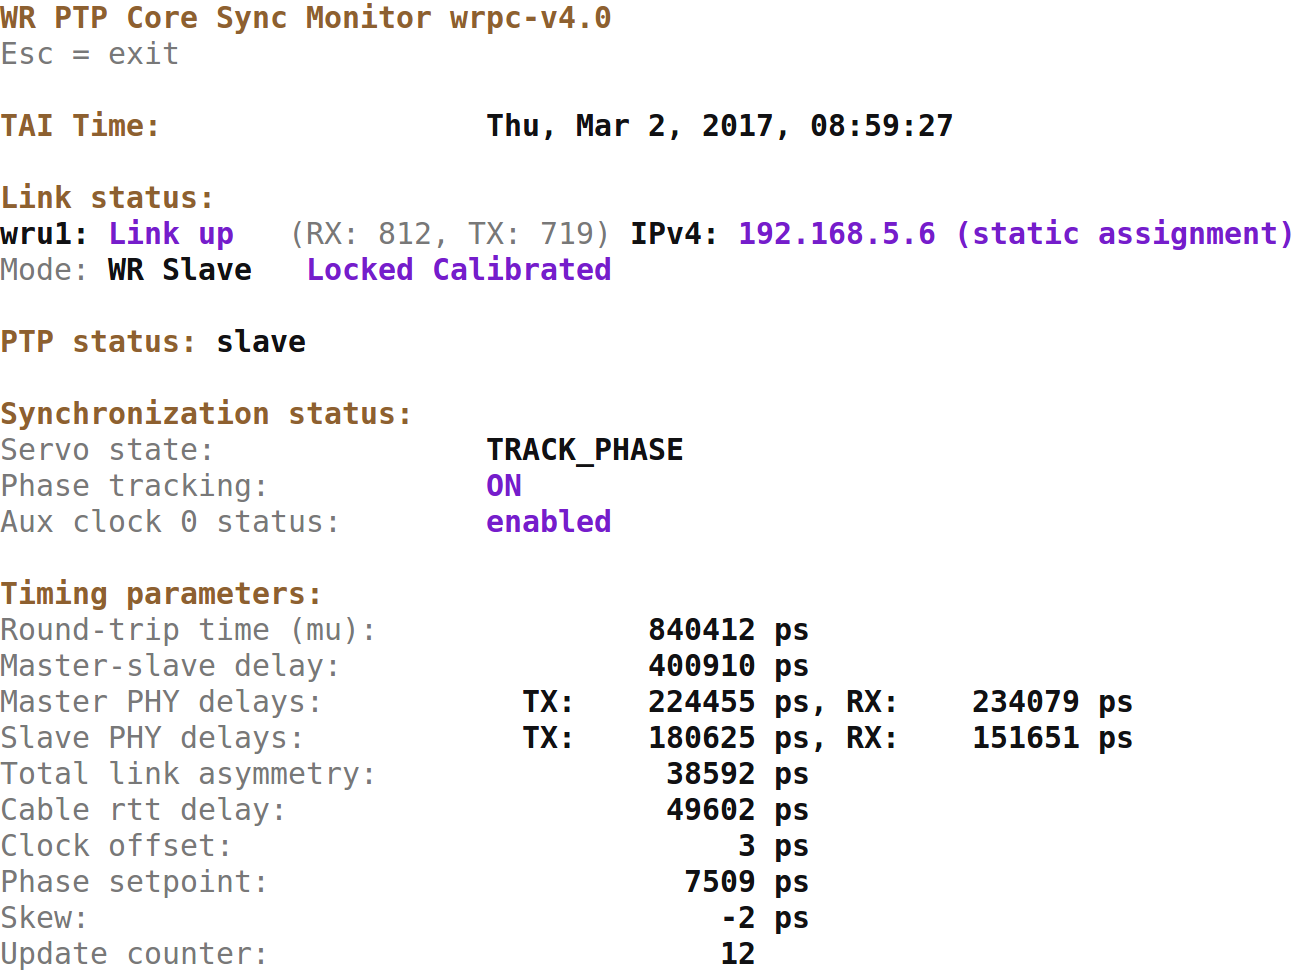
\includegraphics[width=12cm]{wrpc_mon.png}
\vspace{1em}

If you want to log statistics from the \codeHook{wrpc} operation, it's probably
better to use the \textit{stat} shell command. It reports the same information as GUI
but in a single long line, a form which is easier to parse and analyze:

\begin{lstlisting}
wrc# stat
lnk:1 rx:416 tx:118 lock:1 sv:1 ss:'TRACK_PHASE' aux:0 sec:94197 \
nsec:793068184 mu:836241 dms:400556 dtxm:10 drxm:163610 dtxs:0 drxs:128400 \
asym:35129 crtt:544221 cko:-5 setp:7667 hd:61479 md:37221 ad:65000 ucnt:101 \
temp: 45.6875 C
lnk:1 rx:417 tx:119 lock:1 sv:1 ss:'TRACK_PHASE' aux:0 sec:94198 \
nsec:293076296 mu:836253 dms:400562 dtxm:10 drxm:163610 dtxs:0 drxs:128400 \
asym:35129 crtt:544233 cko:-4 setp:7663 hd:61485 md:37259 ad:65000 ucnt:102 \
temp: 45.6875 C
(...)
\end{lstlisting}

\vspace{1em}
Unlike \textit{gui}, the \textit{stat} command runs asynchronously: you can still
issue shell commands while stats are running (this is different from
earlier \texttt{wrpc-sw} releases).  You can stop statistics by running \textit{stat} again.
As an alternative to the toggling action of \textit{stat} alone, you can
use ``\textit{stat 1}'' or ``\textit{stat 0}''.

Statistics are printed every time the WR servo runs; thus no statistics
are reported when the node is running in master mode, nor when your node
is running as slave and the master disappeared.

\vspace{1em}
If you have a \codeHook{dio} mezzanine board plugged to your \codeHook{spec}, you can verify
the synchronization performance by observing the offset between 1-PPS signals
from the \codeHook{wr} Master and \codeHook{wr} Slave. The \codeHook{wr ptp core} generates 1-PPS
signal on the LEMO connector No. 1. Please remember to use oscilloscope cables
of the same length and type (with the same delay), or take their delay
difference into account in your measurements.


% ==========================================================================
\subsection{Diagnostics via SNMP}
\label{Diagnostics via SNMP}

Up to the version 3.1 of \codeHook{wrpc} the only way to perform diagnostics
of the \texttt{wrpc-sw} was to use serial console with tools like \textit{gui}, \textit{stat},
etc. For some set-ups, like standalone node, it is very inconvenient to use
external console for diagnostics.

From the version 3.1 of \codeHook{wrpc} it is possible to include the \textit{Mini
SNMP responder}, which allows to perform remote diagnostics using \textit{SNMP} via
a port connected to the \textit{Write Rabbit} network.

The configuration file of \codeHook{wrpc} contains the following
SNMP-related options:
\begin{itemize*}
\item \texttt{CONFIG\_SNMP} -- include the \textit{Mini SNMP responder} into \codeHook{wrpc}
\item \texttt{CONFIG\_SNMP\_SET} -- enable the support of SNMP \textit{SET} packets
\item \texttt{CONFIG\_SNMP\_VERBOSE} -- enable verbose output from the \textit{Mini SNMP
      responder} on the \codeHook{wrpc}'s console
\end{itemize*}

The MIB file describing \codeHook{wrpc}'s OIDs can be found in the \texttt{lib} directory
of the \texttt{wrpc-sw} repo.
So far, the \textit{Mini SNMP responder} supports version 1 and a subset of version
2c of the SNMP protocol.
The following types of requests are supported:
\begin{itemize*}
   \item GET -- get value of a given OID
   \item GETNEXT -- get value of a next OID after the given OID (this is used
         for \texttt{snmpwalk}s)
   \item SET -- change the value of a given OID (so far used only for adding
         SFP's to the database and PTP restarts)
\end{itemize*}
The \textit{Mini SNMP responder} does not support:
\begin{itemize*}
   \item bulk requests packets (GETBULK)
   \item more than one OID in the request packet
   \item \texttt{trap} and \texttt{inform} packets
   \item encryption
   \item authentication
   \item SNMPv2c return error types; all returned error types follows SNMPv1
\end{itemize*}
To make examples more readable, listings below use \texttt{SNMP\_OPT} environment
variable. Make sure you set it properly in your shell.
\begin{lstlisting}
 $ SNMP_OPT="-c public -v 2c -m WR-WRPC-MIB -M +/var/lib/mibs/ietf:lib \
   192.168.1.20"
\end{lstlisting}
where:
\begin{sloppypar} % to prevent \texttt{} from going to the margine
\begin{itemize*}
   \item \texttt{-c public} -- sets SNMP community as "\textit{public}"
   \item \texttt{-v 2c} -- specifies SNMP version
   \item \texttt{-m WR-WRPC-MIB} -- specifies MIBs to be loaded
   \item \texttt{-M +/var/lib/mibs/ietf:lib} -- contains path to MIBs in the host
         system (\texttt{/var/lib/mibs/ietf}) and path to \texttt{WR-WRPC-MIB} (\texttt{lib});
         on Debian-like systems default MIBs can be downloaded using
         \texttt{download-mibs} command (package \texttt{snmp-mibs-downloader}); on
         CentOS and RedHat MIBs are included in the \texttt{libsmi} package
   \item \texttt{192.168.1.20} -- the IP address of the target board
\end{itemize*}\end{sloppypar}\noindent
For example, to get the system uptime please execute the \texttt{snmpget} command:
\begin{lstlisting}
 $ snmpget $SNMP_OPT wrpcTimeSystemUptime.0
\end{lstlisting}
To get dump of all available OIDs please execute the \texttt{snmpwalk} command:
\begin{lstlisting}
 $ snmpwalk $SNMP_OPT wrpcCore
\end{lstlisting}
Part of the \texttt{snmpwalk}'s output:
\begin{lstlisting}
 WR-WRPC-MIB::wrpcVersionHwType.0 = STRING: spec
 WR-WRPC-MIB::wrpcVersionSwVersion.0 = STRING: wrpc-v3.0-251-g14e952e
 WR-WRPC-MIB::wrpcVersionSwBuildBy.0 = STRING: Adam Wujek
 WR-WRPC-MIB::wrpcVersionSwBuildDate.0 = STRING: Jun  7 2016 18:12:24
 WR-WRPC-MIB::wrpcTimeTAI.0 = Counter64: 1465375022
 WR-WRPC-MIB::wrpcTimeTAIString.0 = STRING: 2016-06-08-08:37:02
 WR-WRPC-MIB::wrpcTimeSystemUptime.0 = Timeticks: (18186) 0:03:01.86
 WR-WRPC-MIB::wrpcTemperatureName.1 = STRING: pcb
 WR-WRPC-MIB::wrpcTemperatureValue.1 = STRING: 38.5625
 WR-WRPC-MIB::wrpcSpllMode.0 = INTEGER: slave(3)
 WR-WRPC-MIB::wrpcSpllIrqCnt.0 = Counter32: 1259605
 [...]
 WR-WRPC-MIB::wrpcPortSfpInDB.0 = INTEGER: inDataBase(2)
 WR-WRPC-MIB::wrpcPortInternalTx.0 = Counter32: 452
 WR-WRPC-MIB::wrpcPortInternalRx.0 = Counter32: 869
 WR-WRPC-MIB::wrpcSfpPn.1 = STRING: AXGE-1254-0531
 WR-WRPC-MIB::wrpcSfpDeltaTx.1 = INTEGER: 180625
 WR-WRPC-MIB::wrpcSfpDeltaRx.1 = INTEGER: 148451
 WR-WRPC-MIB::wrpcSfpAlpha.1 = INTEGER: 72169888
 End of MIB
\end{lstlisting}

It is recommended to use SNMP v2c for communication with the \codeHook{wrpc}.
Please note that when the version 1 of SNMP is used, 64 bit counters are not
supported. This makes it impossible to read some \codeHook{wrpc}'s objects with
SNMPv1.

% --------------------------------------------------------------------------
\subsubsection{Managing SFP database via SNMP}
\label{Managing SFP database via SNMP}

The SFPs database can be displayed using the \texttt{sfp show} command from
the \codeHook{wrpc}'s console:
\begin{lstlisting}
 wrc# sfp show
 1: PN:AXGE-1254-0531   dTx:   180625 dRx:   148451 alpha: 72169888
 2: PN:AXGE-3454-0531   dTx:   180625 dRx:   148451 alpha: -73685416
\end{lstlisting}
The same data is exported by the \textit{Mini SNMP responder} via the table
\texttt{wrpcSfpTable}:

\begin{lstlisting}
 $ snmpwalk $SNMP_OPT wrpcSfpTable
 WR-WRPC-MIB::wrpcSfpPn.1 = STRING: AXGE-1254-0531
 WR-WRPC-MIB::wrpcSfpPn.2 = STRING: AXGE-3454-0531
 WR-WRPC-MIB::wrpcSfpDeltaTx.1 = INTEGER: 180625
 WR-WRPC-MIB::wrpcSfpDeltaTx.2 = INTEGER: 180625
 WR-WRPC-MIB::wrpcSfpDeltaRx.1 = INTEGER: 148451
 WR-WRPC-MIB::wrpcSfpDeltaRx.2 = INTEGER: 148451
 WR-WRPC-MIB::wrpcSfpAlpha.1 = INTEGER: 72169888
 WR-WRPC-MIB::wrpcSfpAlpha.2 = INTEGER: -73685416
 End of MIB
\end{lstlisting}
When the SET support is compiled into the \textit{Mini SNMP responder}, it is
possible to erase or add/replace SFP entires to the SFPs database via SNMP.

\begin{sloppypar} % to prevent \texttt{} from going to the margine
Addition (or modification) of one SFP to the database can done by a row of
SNMP SETs. Firstly, please set the delta Tx (\texttt{wrpcPtpConfigDeltaTx.0}), the
delta Rx (\texttt{wrpcPtpConfigDeltaRx.0}) and the alpha (\texttt{wrpcPtpConfigAlpha.0})
with new values.
Then, to commit the change to the SFP database, perform the SNMP SET on
the \texttt{wrpcPtpConfigApply.0} with the value \texttt{writeToFlashCurrentSfp}. It will
add/update values for the currently plugged SFP.
\end{sloppypar}

To add/update entries for different SFPs, please set deltas and alpha like
above, then set PN of an SFP to the \texttt{wrpcPtpConfigSfpPn.0} and commit
the change by setting \texttt{writeToFlashGivenSfp} to the \texttt{wrpcPtpConfigApply.0}.

It is also possible to update values in the memory for the current SFP.
For that, please set delta Tx, delta Rx and alpha as described above,
then set \texttt{writeToMemoryCurrentSfp} to the \texttt{wrpcPtpConfigApply.0}

Please be aware that these changes will be lost after a power cycle of a board,
soft reset of \codeHook{wrpc} or unplug/plug of a fiber/SFP.

Currently, after the update of SFP values in the memory, PTP is restarted.
Such restart is necessary because PTP does not support on-the-fly changes of
deltas nor alpha. It is expected that this behavior will change in the future.

If a database entry of the SFP, which is currently used was updated, it is
necessary to perform a restart of the PTP daemon
(set \texttt{wrpcPtpConfigRestart.0} with the value \texttt{restartPtp}).

Each SNMP SET of \texttt{wrpcPtpConfigApply.0} or \texttt{wrpcPtpConfigRestart.0} returns
the status of a performed action. For details please check \texttt{WR-WRPC-MIB}
file.

Commands below add an SFP with PN as "\texttt{NEW-SFP}", delta Tx "\texttt{1111}",
delta Rx "\texttt{2222}" and alpha "\texttt{3333}".
\begin{lstlisting}
 $ snmpset $SNMP_OPT wrpcPtpConfigDeltaTx.0 = 1111
 WR-WRPC-MIB::wrpcPtpConfigDeltaTx.0 = INTEGER: 1111
 $ snmpset $SNMP_OPT wrpcPtpConfigDeltaRx.0 = 2222
 WR-WRPC-MIB::wrpcPtpConfigDeltaRx.0 = INTEGER: 2222
 $ snmpset $SNMP_OPT wrpcPtpConfigAlpha.0 = 3333
 WR-WRPC-MIB::wrpcPtpConfigAlpha.0 = INTEGER: 3333
 $ snmpset $SNMP_OPT wrpcPtpConfigSfpPn.0 = NEW-SFP
 WR-WRPC-MIB::wrpcPtpConfigSfpPn.0 = STRING: "NEW-SFP"
 $ snmpset $SNMP_OPT wrpcPtpConfigApply.0 = writeToFlashGivenSfp
 WR-WRPC-MIB::wrpcPtpConfigApply.0 = INTEGER: applySuccessful(100)
\end{lstlisting}

In case the SFP database does not contain the currently plugged SFP, the last
\texttt{snmpset} command will return \texttt{applySuccessfulMatchFailed(101)}.

Optionally restart the PTP:
\begin{lstlisting}
 $ snmpset $SNMP_OPT wrpcPtpConfigRestart.0 = restartPtp
 WR-WRPC-MIB::wrpcPtpConfigRestart.0 = INTEGER: restartPtpSuccessful(100)
\end{lstlisting}

Simple verification of performed actions:
\begin{lstlisting}
 wrc# sfp show
 1: PN:AXGE-1254-0531   dTx:   180625 dRx:   148451 alpha: 72169888
 2: PN:AXGE-3454-0531   dTx:   180625 dRx:   148451 alpha: -73685416
 3: PN:NEW-SFP          dTx:     1111 dRx:     2222 alpha:     3333
\end{lstlisting}

The same add can also be achieved by performing \texttt{sfp add} command in
the \codeHook{wrpc}'s console:
\begin{lstlisting}
 wrc# sfp add NEW-SFP 1111 2222 3333
 Update existing SFP entry
 3 SFPs in DB
\end{lstlisting}

Verify the result via SNMP:
\begin{lstlisting}
 $ snmpwalk $SNMP_OPT wrpcSfpTable
 WR-WRPC-MIB::wrpcSfpPn.1 = STRING: AXGE-1254-0531
 WR-WRPC-MIB::wrpcSfpPn.2 = STRING: AXGE-3454-0531
 WR-WRPC-MIB::wrpcSfpPn.3 = STRING: NEW-SFP
 WR-WRPC-MIB::wrpcSfpDeltaTx.1 = INTEGER: 180625
 WR-WRPC-MIB::wrpcSfpDeltaTx.2 = INTEGER: 180625
 WR-WRPC-MIB::wrpcSfpDeltaTx.3 = INTEGER: 1111
 WR-WRPC-MIB::wrpcSfpDeltaRx.1 = INTEGER: 148451
 WR-WRPC-MIB::wrpcSfpDeltaRx.2 = INTEGER: 148451
 WR-WRPC-MIB::wrpcSfpDeltaRx.3 = INTEGER: 2222
 WR-WRPC-MIB::wrpcSfpAlpha.1 = INTEGER: 72169888
 WR-WRPC-MIB::wrpcSfpAlpha.2 = INTEGER: -73685416
 WR-WRPC-MIB::wrpcSfpAlpha.3 = INTEGER: 3333
 End of MIB
\end{lstlisting}

It is also possible to erase the SFPs database via SNMP (equivalent of
the \texttt{sfp erase} command):
\begin{lstlisting}
 $ snmpset $SNMP_OPT wrpcPtpConfigApply.0 = eraseFlash
 WR-WRPC-MIB::wrpcPtpConfigApply.0 = INTEGER: applySuccessful(100)
\end{lstlisting}

To verify that database is empty:
\begin{lstlisting}
 wrc# sfp show
 SFP database empty
\end{lstlisting}

% --------------------------------------------------------------------------
\subsubsection{Adding new objects to the SNMP}
\label{Adding new objects to the SNMP}

The \textit{Mini SNMP responder} can be easily expanded to export new objects.
Values of new objects can come from \codeHook{wrpc}'s variables or other HDL modules
as long as there is a proper interface to the \codeHook{wrpc} to read these values.

This section contains the instruction how to export new objects with
the given variables' content.

The \textit{Mini SNMP responder} internally divides all OIDs into two parts.
The first part is called \textit{limb}. The \textit{limb} part of the incoming OID is
matched by a function \texttt{snmp\_respond}, with the defined \textit{limb} parts of OIDs
in the structure \texttt{oid\_limb\_array}.
When the \textit{limb} part is matched then the corresponding function from
the structure \texttt{oid\_limb\_array} is called to try to match the second part of
OID (the \textit{twig} part).

\begin{sloppypar} % to prevent \texttt{} from going to the margine
The example below adds to the \textit{Mini SNMP responder} an \texttt{int32\_t} variable
(\texttt{example\_i32var}) with OID \texttt{1.3.6.1.4.1.96.102.1.1.0} and a string
(\texttt{example\_string}) with OID \texttt{1.3.6.1.4.1.96.102.1.2.0}.
Before assigning new OIDs in your projects please contact the maintainer of
\texttt{wrpc-sw} repo to avoid conflicts.
\end{sloppypar}

\begin{itemize*}
\item First declare \texttt{example\_i32var} and \texttt{example\_string}:
\begin{lstlisting}
 static int32_t example_i32var;
 static char example_string[] = "test string";
\end{lstlisting}

\item Define the \textit{limb} part of the OID:
\begin{lstlisting}
 static uint8_t oid_wrpcExampleGroup[] = {0x2B,6,1,4,1,96,101,99};
\end{lstlisting}

\item Define the \textit{twig} part of the OID:
\begin{lstlisting}
 static uint8_t oid_wrpcExampleV1[] = {1,0};
 static uint8_t oid_wrpcExampleV2[] = {2,0};
\end{lstlisting}

\item Add a group definition to the \texttt{struct snmp\_oid\_limb oid\_limb\_array}.
      Please note that this structure has to be sorted by ascending OIDs.
\begin{lstlisting}
OID_LIMB_FIELD(oid_wrpcExampleGroup, func_group, oid_array_wrpcExampleGroup),
\end{lstlisting}
The macro \texttt{OID\_LIMB\_FIELD} takes the following arguments:
\begin{itemize*}
   \item \texttt{oid\_wrpcExampleGroup} -- an array with the \textit{limb} part of the
         OID
   \item \texttt{func\_group} -- a function to be called when the \textit{limb} part of
         the OID is matched; this function will try to match the \textit{twig} part
         of the OID within a table or a group.
   \item \texttt{oid\_array\_wrpcExampleGroup} -- an array of \textit{twig} parts of OIDs
\end{itemize*}
\item Declare a previously used \texttt{oid\_wrpcExampleGroup}. Please note that
      this structure has to be sorted by ascending \textit{twig} part of OIDs.
\begin{lstlisting}
 static struct snmp_oid oid_array_wrpcExampleGroup[] = {
   OID_FIELD_VAR(oid_wrpcExampleV1, get_p, set_p, ASN_INTEGER,   &example_i32var),
   OID_FIELD_VAR(oid_wrpcExampleV2, get_p, set_p, ASN_OCTET_STR, &example_string),
   { 0, }
 };
\end{lstlisting}
The macro \texttt{OID\_FIELD\_VAR} takes the following arguments:
\begin{itemize*}
   \item \texttt{oid\_wrpcExampleV1} -- an array with \textit{twig} part of the OID
   \item \texttt{get\_p} (or \texttt{get\_pp)} -- a function to be called when \textit{twig}
         part of the OID is matched for SNMP GET requests;
   \item \texttt{set\_p} (or \texttt{set\_pp)} -- a function to be called when a \textit{twig}
         part of the OID is matched for SNMP SET requests; if no SET
         functionality is planned, please use NULL
   \item \texttt{ASN\_INTEGER, ASN\_OCTET\_STR} -- type of the OID; please
         check the source for other possible types
   \item \texttt{\&example\_i32var, \&example\_string} -- addresses to the data in
         memory
\end{itemize*}
In case the address of variables is not known at boot, it is possible to define
a pointer to the variable which will be initialized (e.g. in the \texttt{snmp\_init}
the function) at the boot time. In that case function \texttt{get\_pp} (\texttt{set\_pp}) has
to be used instead of \texttt{get\_p} (\texttt{set\_p}). For variables that are a part of
a structure and have to be accessed via a pointer, a macro \texttt{OID\_FIELD\_STRUCT}
is available.

For more complex extraction of variables or run-time value corrections,
it is possible to use a custom \textit{get} function. It is possible to pass
a constant number to the custom function instead of an address. For example:
\begin{lstlisting}
 OID_FIELD_VAR(oid_wrpcPtpServoUpdateTime, get_servo, NO_SET, ASN_COUNTER64, \
               SERVO_UPDATE_TIME),
\end{lstlisting}

\end{itemize*}
Perform a \texttt{snmpwalk} to get new OIDs:
\begin{lstlisting}
 $ snmpwalk -On $SNMP_OPT 1.3.6.1.4.1.96.102.1
 .1.3.6.1.4.1.96.102.1.1.0 = INTEGER: 123432
 .1.3.6.1.4.1.96.102.1.2.0 = STRING: "test string"
 End of MIB
\end{lstlisting}
Trying to set too long string into the \texttt{example\_string} results in an error:
\begin{lstlisting}
 $ snmpset -On $SNMP_OPT 1.3.6.1.4.1.96.102.1.2.0 s "new long string"
 Error in packet.
 Reason: (badValue) The value given has the wrong type or length.
 Failed object: .1.3.6.1.4.1.96.102.1.2.0
\end{lstlisting}
A short enough (not longer than defined \texttt{"test string"}) value succeeds:
\begin{lstlisting}
 $ snmpset -On $SNMP_OPT 1.3.6.1.4.1.96.102.1.2.0 s "new value12"
 .1.3.6.1.4.1.96.102.1.2.0 = STRING: "new value12"
\end{lstlisting}
Set 999 to the \texttt{example\_i32var}:
\begin{lstlisting}
$ snmpset -On $SNMP_OPT 1.3.6.1.4.1.96.102.1.1.0 i 999
.1.3.6.1.4.1.96.102.1.1.0 = INTEGER: 999
\end{lstlisting}
Perform \texttt{snmpwalk} to verify changes:
\begin{lstlisting}
$ snmpwalk -On $SNMP_OPT 1.3.6.1.4.1.96.102.1
.1.3.6.1.4.1.96.102.1.1.0 = INTEGER: 999
.1.3.6.1.4.1.96.102.1.2.0 = STRING: "new value12"
End of MIB
\end{lstlisting}

% --------------------------------------------------------------------------
\subsubsection{Mini SNMP responder's tests}
\label{Mini SNMP responder's tests}

In the \texttt{wrpc-sw} repo, automatic tests are available to validate the \textit{Mini
SNMP responder} implementation. These tests are placed in the \texttt{test/snmp}
directory.
They use the \texttt{bats} framework (\url{https://github.com/sstephenson/bats}).

To run these tests, please go to \texttt{test/snmp} directory, then set
\texttt{TARGET\_IP} environment varaible to the IP of your target board, then type
\texttt{make}. For example:
\begin{lstlisting}
 $ TARGET_IP=192.168.1.20 make
 bats/libexec/bats snmp_tests_*.bats
   Host up 192.168.1.20
   Check the presence of snmpget
   Check the presence of snmpgetnext
   Check the presence of snmpwalk
   Check the presence of snmpset
   snmpget existing oid 1.3.6.1.4.1.96.101.1.1.1.0
 [...]
   snmpwalk 1.3.6.1.4.1.95
   snmpwalk 1.3.6 count all OIDs
 100 tests, 0 failures
\end{lstlisting}
On the left of each test there will be a tick symbol shown or an \texttt{x}
depending of the test's result (not included in the example above).

Be aware that it might be necessary to clone the \texttt{bats} repo first.
\texttt{make} command will inform whether this is needed.

In case the number of OIDs changes please correct variable \texttt{TOTAL\_NUM\_OIDS}
in file \texttt{snmp\_test\_config.bash}.

These tests have to be executed after any changes are made to the \textit{Mini SNMP
responder}.

% ==========================================================================
\subsection{Other Diagnostic Tools}
\label{Other Diagnostic Tools}

% --------------------------------------------------------------------------
\subsubsection{Syslog}
\label{Syslog}

\begin{sloppypar} % to prevent \texttt{} from going to the margine
The node can act as a \textit{syslog} client, though only on the UDP protocol.
To activate it, you must build with \texttt{CONFIG\_SYSLOG} and pass proper
parameters at run time.

To configure \textit{syslog} you can run the \texttt{syslog} shell command, which
receives two parameters (\texttt{ipaddr} and \texttt{macaddr}), or the
single \texttt{off} subcommand.

When deploying a network of nodes, you can choose to put the \texttt{syslog
<ip> <mac>} command in the build-time init command. To this aim you
must activate \texttt{CONFIG\_BUILD\_INIT} and then pass your command string
as \texttt{CONFIG\_INIT\_COMMAND}.  In that context, you can use ``\texttt{;}'' as
a command separator, as no newlines are permitted in \texttt{Kconfig}
strings.

The strings that a WR node sends to the \textit{syslog} server are always
using the format:  ``\texttt{<}\textit{level}\texttt{>} \textit{Jan 01 00:00:00 192.168.1.1 msg}''
where \textit{level} is usually 14 (type ``user'', priority ``info'')
and \textit{msg} is a free-format message strings.
The \textit{syslog} client sends strings to the server in the following
situations:
\begin{longtable}{  p{6.5cm}  p{9cm} }

\textit{ Boot time } &

	The node sends ``\texttt{(ma:ca:dd:rr:ee:ss) Node up since} \textit{X}
        \texttt{seconds}'' as soon as the network link is up and the \textit{syslog}
        server is configured with the shell command or init script.
        The message is re-sent, with an updated uptime value, if you change
        the \textit{syslog} server parameters. \\
& \\
\textit{ Link up after link down } &

	The message is ``\texttt{"Link up after} \textit{2.345} \texttt{s}''. The
        time printed is the duration of the link-down interval just
        passed -- no lost-by-design message is sent at link-down time. The
        message is not sent the first time the link goes up, because
        the boot message is already there.\\
& \\
\textit{ Synchronization, first time } &

	When the node reaches WR synchronization (i.e. ``track phase''
        state), it sends ``\texttt{Tracking after} \textit{5..678} \texttt{s}''.
        The reported time is the lapse since power-on.\\
& \\
\textit{ Synchronization lost } &

	Whenever WR looses \textit{track-phase} status, the node reports
        \texttt{Lost track}.\\
& \\
\textit{ Synchronization recovered } &

	When the WR servo is in \textit{track phase} state after loosing
        synchronization, the node sends ``\textit{45}\texttt{-th re-track after}
        \textit{23.456} \texttt{s}''. The time reported is the amount of time
        during which the node has not been synchronized. The seconth and
        thirth re-sync are reported as \texttt{2-th} and \texttt{3-th}, to make you
        smile. At the \texttt{4-th} you should stop smiling and be concerned.\\
& \\
\textit{ Temperature over threshold } &

	The node monitors the various thermometers every few seconds.
        If \texttt{CONFIG\_TEMP\_POLL\_INTERVAL} and related parameters are
        set, any over-temperature event is reported to \textit{syslog}.
        If any temperature in the collected set is over threshold,
        the message is ``\texttt{Temperature high:}'' followed by the list of
        all collected temperatures.  The message is repeated every
        few seconds (\texttt{CONFIG\_TEMP\_HIGH\_RAPPEL}, default 60)
        until all temperatures are under-threshold. When temperature
        is recovered the node sends ``\texttt{Temperature ok:}'' followed by
        the current list of temperatures.\\

\end{longtable}
\end{sloppypar}

% FIXME: syslog examples

% --------------------------------------------------------------------------
\subsubsection{Latency Test}
\label{Latency Test}

\begin{sloppypar} % to prevent \texttt{} from going to the margine
The configuration choice \texttt{CONFIG\_LATENCY\_PROBE} activates a
mechanism for \textit{wr} nodes to measure network latency, base on the same
hardware timestamps that are used for synchronization -- the mechanism
assumes the nodes are synchronized.

\textit{ltest} frames can be used to verify whether the network is
overloaded and/or has strange inconsistencies in node-to-node delays.

\textit{ltest} frames use a special ethernet type, \texttt{CONFIG\_LATENCY\_ETHTYPE},
which defaults to 0x0123 (291). If \textit{vlans} are active, these frames
are sent and received in the same \textit{vlans} as other CPU frames.

The \texttt{ltest} sender periodically sends three frames, with a sequence
number. One frames is at priority 7, one is at priority 6, and one is
at priority 0. The last frames reports the departure timestamps of the
previous frames.  The \textit{ltest} receiver uses ingress timestamps to
measure latency and report lost frames.

Every node built with \texttt{CONFIG\_LATENCY\_PROBE} listens for frames
belonging to \texttt{CONFIG\_LATENCY\_ETHTYPE}.  A single node in the
network is expected to send \textit{ltest} frames; use the \texttt{ltest}
shell command to select how often to send an \textit{ltest} tuple of three
frames. To enable sending every second use ``\texttt{ltest 1}'', to enable
sending every 100ms use ``\texttt{ltest 0 100}'', to stop sending use
\texttt{ltest 0}.

In the sender node, a reminder is sent to the console very 10s
reporting the node is currently sendin \textit{ltest} frames.  All
non-sending nodes report every minute to \textit{syslog}. The
report message includes the number of samples received as well
as the minimum, average and maximum latency, in nanoseconds.
Any lost frames are reported both to the console and to \textit{syslog}.

You can use \textit{ltest} without \texttt{CONFIG\_SYSLOG}. In that case the
receiver nodes print the exact latency (picosecond resolution) for
every received event.
\end{sloppypar}

% --------------------------------------------------------------------------
\subsubsection{wrpc-dump}
\label{wrpc-dump}

When trying to diagnose software issues, especially lockup situations,
it may be useful to look at the current values or critical variables
within \textit{wrpc-sw}/\textit{ppsi}.

To this aim, you can pass a memory image of \textit{wrpc} to \texttt{tools/wrpc-dump}.
The tools will print information for softpll, ppsi data structures
and ptp data sets.

For example, for a \textit{spec} device, you can use the resource file in
\textit{syfs} to look at a live system, or copy the file for off-line
analysis. The following command line show both uses:

\begin{lstlisting}
   # Look for "resource0" in /sys/devices/pci, choose your bus number.
   FILE=/sys/devices/pci0000:00/0000:00:04.0/0000:04:00.0/resource0

   sudo ./tools/wrpc-dump $FILE

   sudo tools/mapper $FILE 0 0x20000 > wrpc-memory-image
   ./tools/wrpc-dump wrpc-memory-image
\end{lstlisting}

The \textit{mapper} tool used above, and part of \textit{wrpc-sw}, reads a file
using \textit{mmap()}. The kernel doesn't allow plain \textit{read()} from a
resource file.

\textbf{Note:} Data read by \texttt{mapper} may look like has wrong endianness comparing
to the file used for programming lm32 by \texttt{spec-cl}, but \texttt{spec-cl} is the
one which change the endianness of the binary data during the programming.

With \textit{etherbone}, you can get a snapshot for \textit{wrpc} memory using
\texttt{eb-get} and the proper address (the size is always 128kB)

\begin{lstlisting}
   eb-get dev/wbm2 0x4040000/0x20000 wrpc-memory-image
   eb-get dev/ttyUSB2 0x4040000/0x20000 wrpc-memory-image
\end{lstlisting}

We won't show the 180 output lines here, to save some paper, but they
are readable dumps of the data structures, including the PTP timestamps.

% --------------------------------------------------------------------------
\subsubsection{Softpll Timing}
\label{spll Softpll Timing}

To help understanding the CPU time spent in the \textit{softpll}, you can
set \texttt{CONFIG\_SPLL\_FIFO\_LOG} in the configuration. The option
depends on \texttt{CONFIG\_DEVELOPER} and is disabled by default, because
it costs half a kilobyte in binary size and Adam is scared about any size
increase.

When the configuration option is set, \texttt{wrpc-dump} will also show
information about the last 16 \textit{softpll} iterations. Both the \texttt{tstamp}
and \texttt{duration} fields come from reading the \texttt{PPSG} nanosecond counter.

\begin{lstlisting}
   fifo log at 0x17258
        trr:                           0x0126d921
        tstamp:                        0x06b58d6a
        duration:                      0x00000c7e
        irq_count:                     2305
        tag_count:                     2304
        [... repeats for 5 more events ...]
\end{lstlisting}

% --------------------------------------------------------------------------
\subsubsection{Uptime Counter}
\label{Uptime Counter}

\textit{Wrpc-sw} now maintains an ``uptime'' counter, in seconds. It lives
at binary address 0xa0. It can be queried by \textit{etherbone}, or
seen in memory maps.

In addition to know how much as the node been up, it can be used to
know roughly when a node got stuck, and whether software is still
running when a node is not active on the network. Neither of this even
happens in production, but the tool is useful during development.

% --------------------------------------------------------------------------
\subsubsection{Profiling}
\label{Profiling}

The node now has a \textit{ps} command, that shows the number of iterations
and time spent in each \textit{task}. Each task reports when it did
something (as opposed to just polling the clock or network socket and
see nothing is there to do); the \textit{iterations} count shouws how many
times the task did something.

\begin{lstlisting}
   wrc# ps
    iterations     seconds.micros    name
      44288501        4242.816329  idle
             0           0.000000  spll-bh
            37           0.016549  shell+gui
          8992           1.158969  ptp
          4252           0.037005  uptime
             1           0.001035  check-link
             0           0.000000  stats
             0           0.000000  net-bh
           568           5.068343  temperature
\end{lstlisting}

By using ``\texttt{ps reset}'' you can zero all counters to start a new
test run.

% --------------------------------------------------------------------------
\subsubsection{Pfilter rules}
\label{Pfilter rules}

By setting \texttt{CONFIG\_PFILTER\_VERBOSE}, which depends on
\texttt{CONFIG\_DEVELOPER}, you can get a dump of packet-filter rules
whenever they are activated.  This happens at initialization time and
whenever you change the MAC address or \textit{vlan} choice.

% ==========================================================================
\subsection{Network Services}
\label{Network Services}

If built with \texttt{CONFIG\_IP=y}, \textit{wrpc-sw} implements the following
udp-based network services, in addition to \textit{ptp}:

\begin{longtable}{  p{6.5cm}  p{9cm} }

\textit{ bootp } &

	The node will get an IPV4 address by making \textit{bootp} queries
        once per second, until it gets a reply from a server. As an
        alternative, the address can be set using the shell command,
        and in this case the node won't send \textit{bootp} queries, or will
        stop sending them.\\
& \\
\textit{ rdate } &

	The node can be queried using \texttt{rdate -u}, once it has an IP
        address.\\
& \\
\textit{ syslog } &

	If \texttt{CONFIG\_SYSLOG} is set, the node is a syslog client.
        See section \ref{Syslog} for details.\\

\end{longtable}

% ==========================================================================
\subsection{VLAN Support}
\label{VLAN Support}

The White Rabbit node can be configured to be vlan-aware, by setting
\texttt{CONFIG\_VLAN} in \textit{Kconfig}.  The setting depends on \texttt{CONFIG\_DEVELOPER}.

If configured for \textit{vlan} support, the node select packet-filter rules
to receive frames in several \textit{vlan}s, all set at configuration time.

At run time you can use \texttt{vlan off} in the shell to turn off all \textit{vlan}
processing and get back to the ``standard'' packet-filter rules.

\begin{longtable}{  p{6.5cm}  p{9cm} }

\textit{ CONFIG\_VLAN } &

	This is the top-level choice. It can be enabled or disabled.
        If disabled, the following values default to 0 and the
        packet filter will discard all tagged frames.\\
& \\
\textit{ CONFIG\_VLAN\_NR } &

	The default \textit{vlan} number for the CPU.  All network traffic
        directed to (and originating from)the \textit{lm32} processor will
        belong to this \textit{vlan}.  The value can be changed at run time
        using the \texttt{vlan} shell command.\\
& \\
\textit{ CONFIG\_VLAN\_1\_FOR\_CLASS7 } & \\
\textit{ CONFIG\_VLAN\_2\_FOR\_CLASS7 } &

	The packet-filter rules are setup to deliver frames belonging
        to two specific \textit{vlans} to class 7, usually \textit{etherbone}.
        To deliver one \textit{vlan} only, set the two options to the same
        number.\\
& \\
\textit{ CONFIG\_VLAN\_FOR\_CLASS6 } &

	The packet-filter rules are setup to deliver frames belonging
        to one specific \textit{vlan} to class 6, usually routed to the
        \textit{streamer} or \textit{nic} logic blocks.\\

\end{longtable}

% ##########################################################################
\section{Troubleshooting}
\label{Troubleshooting}

\textbf{My computer hangs on loading spec.ko or fmc-trivial.ko driver.}

This will occur when you try to load the driver while your \textit{spec-vuart} is
running and trying to get messages from Virtual-UART's registers inside the
\codeHook{wrpc}. Please remember to quit \textit{spec-vuart} before reloading the driver.

\vspace{1em}
\textbf{I want to synthesize \codeHook{wrpc} but hdlmake does nothing, just quits without any
message.}

Please check if you have the Xilinx ISE-related system variables set correctly
(\textit{settings64.sh} script provided by Xilinx sets them) and make sure you have
overwritten the \textit{\$XILINX} variable to:

\begin{lstlisting}
$ export XILINX=/opt/Xilinx/<version>/ISE_DS
\end{lstlisting}

or similar, if your installation folder differs from default.

\vspace{1em}
\textbf{\codeHook{wr ptp core} seems to work but I observe on my oscilloscope that the offset
between 1-PPS signals from \codeHook{wr} Master and \codeHook{wr} Slave is more than 1 ns.}

If you're trying to synchronize the \codeHook{spec} board to \codeHook{wr} Switch please remember to
read the document and perform the \codeHook{wr} Calibration to find out the values of
deltaRx and deltaTx for your firmware. Check if the oscilloscope cables you use
have the same delays (or take the delay difference into account in your
measurements).


% ##########################################################################
\section{Questions, reporting bugs}
\label{Questions}

If you have found a bug, you have problems with the \codeHook{wr ptp core} or one
of the tools used to build and run it, you can write to our mailing list
\code{white\-/rabbit\-/dev@ohwr.org}


% ##########################################################################


\appendix
\clearpage
\section{WRPC Shell Commands}
\label{WRPC Shell commands}

\footnotesize
\begin{longtable}{  p{7.5cm}  p{7cm} }

  \code{help} & lists available commands in this instance of the \codeHook{wrpc} \\
 & \\
  \code{ver} & prints which version of wrpc is running \\
 & \\
  \code{config} & prints the Kconfig file used to build this instance of
\codeHook{wrpc}. It is an optional command, enabled at build time by
\texttt{CONFIG\_CMD\_CONFIG} \\
 & \\
  \code{ps} & prints the list of running tasks (processes) in the CPU.
For each task you get the number of iterations and the CPU time consumed
since boot or last reset of values\\
 & \\
  \code{ps reset} & zeroes the profiling information reported by
the \code{ps} command\\
 & \\
  \code{verbose <digits>} & sets PPSi verbosity. See the PPSi manual
about the meaning of the digits (hint: \texttt{verbose 1111} is a good first bet to
see how the \codeHook{ptp} system is working) \\
 & \\
  \code{pll init <mode> <ref\_channel> <align\_pps>} & manually runs
spll\_init() function to initialize SoftPll \\

  \code{pll cl <channel>} & checks if SoftPLL is locked for the channel\\

  \code{pll sps <channel> <picoseconds>} & sets phase shift for the channel\\

  \code{pll gps <channel>} & gets current and target phase shift for the channel\\

  \code{pll start <channel>} & starts SoftPLL for the channel\\

  \code{pll stop <channel>} & stops SoftPLL for the channel\\

  \code{pll sdac <index> <val>} & sets the dac\\

  \code{pll gdac <index>} & gets dac's value\\
 & \\
  \code{gui} & starts GUI \codeHook{wrpc} monitor\\
 & \\
  \code{stat} & toggles reporting of loggable statistics. You can pass
\texttt{1} or \texttt{0} as argument as an alternative to toggling\\

  \code{stat bts} & prints bitslide value for established \codeHook{wr} Link,
needed by the calibration procedure\\
 & \\
  \code{refresh} & changes the update time period of the gui and stat
commands. Default period is 1 second. If you set the period to 0, the log
message is only generated one time.\\
 & \\
  \code{ptp start} & starts \codeHook{wr ptp} daemon\\

  \code{ptp stop} & stops \codeHook{wr ptp} daemon\\

  \code{ptp e2e} & select end-to-end PTP mechanism. If configured you can set \texttt{p2p} mode, and \texttt{delay}/\texttt{pdelay} as aliases.\\

  \code{ptp master} & force working as master. Alternatives are \texttt{slave} and \texttt{gm} (grandmaster).\\

  \code{ptp <cmd> <cmd> ...} & You can concatenate several of the above sbcommands in a single \texttt{ptp} command. With no arguments, the command reports the current values.\\
 & \\
  \code{mode gm|master|slave} & sets \codeHook{wrpc} to operate as Grandmaster
clock (requires external 10MHz and 1-PPS reference), Master or Slave. After
setting the mode, \texttt{ptp start} must be re-issued\\
 & \\
  \code{calibration} & tries to read t2/4 phase transition value from the
Flash/EEPROM (in \codeHook{wr} Master or GrandMaster mode), or executes the t24p
calibration procedure and stores its result to the Flash/EEPROM (in \codeHook{wr}
Slave mode)\\
 & \\
  \code{time} & prints current time from \codeHook{wrpc}\\

  \code{time raw} &  prints current time in a raw format (seconds, nanoseconds)\\

  \code{time set <sec> <nsec>} & sets \codeHook{wrpc} time\\

  \code{time setsec <sec>} & sets only seconds of the \codeHook{wrpc} time
(useful for setting time in GrandMaster mode, when nanoseconds counter is
aligned to external 1-PPS and 10 MHz)\\

  \code{time setnsec <nsec>} & sets only nanoseconds of the \codeHook{wrpc} time\\
 & \\
  \code{sfp erase} & erases the \codeHook{sfp} database stored in the Flash/EEPROM\\

  \code{sfp add <PN> <deltaTx> <deltaRx> <alpha>} & stores calibration
parameters for \codeHook{sfp} to a file in Flash/EEPROM\\

  \code{sfp show} & prints all \codeHook{sfp} transceivers stored in database\\

  \code{sfp match} & prints the ID of a currently used \codeHook{sfp}
transceiver and tries to load the calibration parameters for it\\
 & \\
  \code{init erase} & erases the initialization script in Flash/EEPROM \\

  \code{init add <cmd>} & adds shell command at the end of the
initialization script\\

  \code{init show} & prints all commands from the script stored in Flash/EEPROM\\

  \code{init boot} & executes the script stored in Flash/EEPROM (the same action is done automatically when \codeHook{wrpc} starts after resetting \codeHook{lm32})\\
 & \\
  \code{mac get} & prints \codeHook{wrpc}'s \codeHook{mac} address\\

  \code{mac getp} & reads the persistent \codeHook{mac} address stored in Flash/EEPROM\\

  \code{mac set <mac>} & sets the \codeHook{mac} address of \codeHook{wrpc}\\

  \code{mac setp <mac>} & stores the persistent \codeHook{mac} address in Flash/EEPROM\\
 & \\
  \code{sdb} & prints devices connected to the Wishbone bus inside \codeHook{wrpc}\\
 & \\
  \code{ip get} & \\

  \code{ip set <ip>} & reports or sets the IPv4 address of the \codeHook{wrpc} (only available if \texttt{CONFIG\_IP} is set at build time\\
 & \\
  \code{vlan} & \\

  \code{vlan set <n>} & reorts or sets the active vlan used for sending/receiving network frames. The command exists only if \texttt{CONFIG\_VLAN} is set.\\
 & \\
  \code{w1} & List onewire devices on the bus\\
 & \\
  \code{w1w <offset> <byte> [<byte> ...]}& \\

  \code{w1r <offset> <len>} & If \texttt{CONFIG\_W1} is set and a OneWire \codeHook{eeprom} exists, write and read data. For writing, \texttt{byte} values are decimal\\
 & \\
  \code{delays}&\\

  \code{delays <tx> <rx>} & Get or set the constant delays in frame transmission, only available if \texttt{CONFIG\_CMD\_LL}. Delays are expressed in picoseconds.\\
 & \\
  \code{devmem <addr>} & \\

  \code{devmem <addr> <value>} & Read or write a 32-bit word from memory and/or FPGA registers. Only available if \texttt{CONFIG\_CMD\_LL}.\\
 & \\
  \code{diag ...} & diagnostics for auxiliary clocks. Only available if \texttt{CONFIG\_AUX\_DIAG}.\\
 & \\
  \code{temp} & Report current temperatures.\\
 & \\
  \code{faketemp} & \\

  \code{faketemp <T1> <T2> <T3>}  & Read or set the three fake temperatures, used to test the temperature/syslog mechanism. Available if \texttt{CONFIG\_FAKE\_TEMPERATURES}.\\
 & \\
  \code{ltest} & \\

  \code{ltest <secs> <msecs>} & Read or set the latency-test sending interval. See \ref{Latency Test}.\\
 & \\
  \code{syslog off} & \\

  \code{syslog <ipaddr> <macaddr>} & Disable or set your \textit{syslog} server. See \ref{Syslog}.\\

\end{longtable}



% ##########################################################################
\clearpage
\section{WRPC GUI elements}
\label{WRPC GUI elements}

\footnotesize
\begin{longtable}{  p{4.5cm}  p{10cm} }

  \code{TAI Time:} & current state of device's local clock \\

  \code{RX:} / \code{TX:} & Rx/Tx packets counters\\

  \code{mode:} & operation mode of the \codeHook{wr ptp core} - \code{<WR Master, WR Slave>}\\

  \code{< Locked, NoLock >} & SoftPLL lock state\\
 & \\

  \code{Servo state:} & current state of \codeHook{wr} servo state machine -
\code{<Uninitialized, SYNC\_SEC, SYNC\_NSEC, SYNC\_PHASE, TRACK\_PHASE>}\\
 & \\

  \code{Phase tracking:} & is phase tracking enabled when \codeHook{wr} Slave is
synchronized to \codeHook{wr} Master - \code{<ON, OFF>}\\

  \code{Synchronization source:} & network interface name from which \codeHook{wr}
daemon gets synchronization - \code{<wru1>}\\
 & \\

  \code{Round\-/trip time (mu):} & round-trip delay in picoseconds
(\( delay_{MM} \))\\
 & \\

  \code{Master\-/slave delay:} & estimated one-way (master to slave) link
delay (\( delay_{MS} \))\\
 & \\

  \code{Master PHY delays:} & transmission/reception delays of \codeHook{wr}
Master's hardware (\( \Delta_{TXM}, \Delta_{RXM} \))\\
 & \\

  \code{Slave PHY delays:} & transmission/reception delays of \codeHook{wr} Slave's
hardware (\( \Delta_{TXS}, \Delta_{RXS} \))\\
 & \\

  \code{Total link asymmetry:} & \codeHook{wr} link asymmetry calculated as
\( delay_{MM} - 2 \cdot delay_{MS} \)\\
 & \\

  \code{Cable rtt delay:} & round-trip fiber latency\\
 & \\

  \code{Clock offset:} & Slave to Master offset calculated by \codeHook{ptp} daemon
(\( offset_{MS} \))\\
 & \\

  \code{Phase setpoint:} & current Slave's clock phase shift value\\
 & \\

  \code{Skew:} & the difference between current and previous estimated
one-way link delay\\
 & \\

  \code{Update counter:} & the state of counter incremented every time
the \codeHook{wr} servo is updated\\
 & \\

\end{longtable}



% ##########################################################################
\clearpage
\section{Writing SDBFS image in standalone configuration}
\label{Writing SDBFS image in standalone configuration}

If you use \codeHook{spec} board in a host-less environment, or you use custom
hardware and \codeHook{spec} drivers and tools cannot be used, there is still a
possibility of writing \codeHook{sdbfs} through Xilinx JTAG.

\vspace{1em}
In case of \codeHook{spec} running a reference bitstream provided with a stable
\codeHook{wrpc} release, you can simply program your Flash with \textit{spec\_top.mcs}
provided with the release binaries using for example Xilinx ISE Impact tool.
This \textit{mcs} file already includes both \codeHook{sdbfs} image and FPGA bitstream.

In case of a custom gateware or hardware, you can download a standalone
\codeHook{sdbfs} image:
\begin{lstlisting}
$ wget http://www.ohwr.org/attachments/download/4144/sdbfs-standalone.bin
\end{lstlisting}
and generate a custom \textit{*.mcs} file with your own FPGA bitstream. You should
use the following layout:
\begin{longtable}{  l  l }
\code{0x000000} & your FPGA bitstream \\
\code{0x170000} & \codeHook{sdbfs} image\\
\end{longtable}

For example, to generate the \textit{*.mcs} file for M25P32 Flash on \codeHook{spec}, the
following \textit{promgen} parameters should be used:
\begin{lstlisting}
promgen -w -spi -p mcs -c FF -s 32768 -u 0 <your_bitstream>.bit \
-bd sdb-standalone.bin start 0x170000 -o output.mcs
\end{lstlisting}

After that, you can use the Xilinx JTAG cable and Xilinx ISE Impact tool to
write your \textit{output.mcs} file to the Flash memory.
\newpage
% ##########################################################################
\section{wrpc-dump with Older WRPC Binaries}
\label{wrpc-dump with Older WRPC Binaries}

The tool has another working mode, that you can use with older
\textit{wrpc} builds, where the special table is missing (but please be
aware that the data structures may have changed slightly).  In this
mode, you provide the address of the data structure and its name. It
supports the names \textit{pll}, \textit{fifo} (the circular log described
above), \textit{ppg}, \textit{ppi}, \textit{servo\_state}, and \textit{ds}. The last name
refers to the PTP data sets, and for this the pointer needed is
\texttt{ppg} (ppsi global data).
This is an example:

\begin{lstlisting}
   $ ./tools/wrpc-dump dump-file 00015798 servo_state

   servo_state at 0x15798
           if_name:                   ""
           flags:                     1
           state:                     4
           delta_tx_m:                10
           delta_rx_m:                174410
           delta_tx_s:                0
           delta_rx_s:                3200
           fiber_fix_alpha:           73622176
           clock_period_ps:           8000
           t1:                        correct 1: 1448628309.390213200:0000
           t2:                        correct 1: 1448628309.390213520:2921
           t3:                        correct 1: 1448628310.419072616:0000
           t4:                        correct 1: 1448628310.419073104:6041
   [...]
\end{lstlisting}

The address is specified as a hex number, and can be retrieved running
``\texttt{lm32-elf-nm  wrc.elf}''.

Please note that the \textit{spec} device has a strange memory mapping, and
it needs a special endian conversion. With current \textit{wrpc} it is
autodetected, but if you dump an older binary you'll need to set the
\texttt{WRPC\_SPEC} environment variable (to any value you like) to properly
access the PCI memory or a dump taken from PCI:
\begin{lstlisting}
   $ export WRPC_SPEC=y
\end{lstlisting}
or
\begin{lstlisting}
   $ WRPC_SPEC=y ./tools/wrpc-dump dump-file 00015798 servo_state
\end{lstlisting}
This is not needed if the dump is retrieved using Etherbone.

% ##########################################################################
%  LocalWords:  gnudd titlepage iftex texinfo CERN documentlanguage settitle
%  LocalWords:  documentencoding setfilename afourpaper paragraphindent FPGA
%  LocalWords:  setchapternewpage finalout gateware ohwr modprobe insmod cset
%  LocalWords:  smallexample ctrl timestamp fdelay struct spusa hdlmake Xilinx
%  LocalWords:  bitstream wrpc init EEPROM grandmaster wrpcsw noposix http
%  LocalWords:  tarball toolchain specsw sudo Etherbone


\end{document}
